%\documentclass[10pt,a4paper]{article}
\documentclass[ShortAfour,times,sageapa]{sagej}
\usepackage[utf8]{inputenc}
\usepackage[T1]{fontenc}
\usepackage{amsmath}
\usepackage{amssymb}
\usepackage{graphicx}
\usepackage{longtable}


\begin{document}
	
\runninghead{Luchman}
\title{Dominance analysis for count regression models}
\author{Joseph N. Luchman\affilnum{1}}
\affiliation{\affilnum{1}Fors Marsh}

\begin{abstract}
	Determining independent variable relative importance is a highly useful practice in organizational science.  Whereas techniques to determine independent variable importance are available for normally distributed and binary dependent variable models, such techniques have not been extended to count dependent variables (CDVs).  The current work extends previous research on binary and multi-category dependent variable relative importance analysis to provide a methodology for conducting relative importance analysis on CDV models using dominance analysis (DA).  Moreover, the current work provides a set of comprehensive data analytic examples that demonstrate how and when to use CDV models in a DA and the advantages general DA statistics offer in interpreting CDV model results.  Moreover, the current work outlines best practices for determining independent variable relative importance for CDVs using replaceable examples on data from the publicly available National Longitudinal Survey of Youth 1979 cohort.  The present work then contributes to the literature by using in-depth data analytic examples to outline best practices in conducting relative importance analysis for CDV models and by highlighting unique information DA results provide about CDV models.
\end{abstract}

\keywords{Dominance Analysis, Relative Importance, Poisson Regression, Negative Binomial Regression, R-square}

\maketitle

\section{Introduction}

	Quantitative research on topics such as job performance, employee wellness, and business strategy often require that organizational researchers use data that are in the form of discrete, sometimes infrequent, events such as number of contracts won in a year, number of complaints received in a month, or number of days absent for illness in a business quarter. % use actual examples here?
	Discrete, infrequent events are commonly encountered as dependent variables in organizational science \cite[e.g.,]{bettinazzi2021stakeholder,naumovska2021strength,soda2021networks} and are modeled using \textit{count regression models/CRMs}   %howto get the 'e.g.,' at the beginning?  Cite Spain et al here?
	However widely used, CRMs are are complicated to interpret.
	The primary complication with interpreting CRMs is that their functional form differs from the simpler Normal or Gaussian distributed linear regression model/LRM that tends to be better understood among organizational scientists.  % do I need to support this statement?
	 
	\textit{Poisson regression/PR} and \textit{negative Binomial regression/NBR} are CRMs that are based on probability distributions suitable for non-negative integer values but are complicated to interpret as they use log-linear link functions (i.e., have the form $e^{\sum\beta x}$) to adapt their predictions to the non-negative range of real numbers \cite{blevins2015count}.
	CRMs have additional complexities as they are often generated as aggregations of events over a specific time period.
	For instance, a count measure might be the number of organizations adopting a specific practice in a time period \cite{naumovska2021strength} or number of divestitures in a year \cite{bettinazzi2021stakeholder}. 
	When the period of aggregation differs across observations in the data, additional \emph{offset} terms are needed to re-establish parity across observations \cite[see, for an example]{glerum2021trainer}.
	Furthermore, some count measures suffer from \emph{zero inflation}; a situation in which there are more 0 values than would be expected from a PR or NBR model and can be remedied by a specialized zero-inflation model \cite[again see, for an example]{glerum2021trainer}.
	
	The complexities of CRM interpretation and additional considerations such as offset terms also affect model postestimation methods such as relative importance analysis. 
	To date, published methodological work on discussed how to apply relative importance analysis to similarly complex models such as binary \cite{azen2009using}, ordered, and multinomial logit models \cite{luchman2014relative} but has not provided an extensive discussion relative importance analysis with CRMs. 
	Relative importance analysis is a widely used model postestimation method used for interpretation that adds detail to the estimation of parameter estimates and can provide practically useful information about independent variable/IV predictive utility \cite{tonidandel2011relative}.  
	Among relative importance analysis methods, \cite[dominance analysis/DA]{azen2003dominance} is most often recommended as a method that has a strong conceptual foundation \cite{gromping2007estimators} and flexible implementation in terms of extensibility \cite[see]{luchman2021determining}.
	
	% ended here
	
	This manuscript extends the literature on CRMs and DA in three ways.
	First, this work provides a discussion of and recommendations for DA as applied to CRMs commonly used in organizational science.
	In discussing how to extend DA do CRMs, a focus will be on recommending the use of a model fit metric that is comparable to those available for LRM.
	Additionally, I will focus on highlighting the similarities between DA results with the well-understood LRM and those obtained with CRMs given an identical structure of the underlying data.
	The similarities between these results are intended to empirically demonstrate the idea that DA can be extended to CRMs and reinforce that the DA methodology is a model agnostic-model free decomposition and importance approach.
	Second, this work focuses on the use of DA for the interpretation of CRMs.  
	In this way, this paper can also be seen as an extension of Blevins, Tsang, and Spain's \cite{blevins2015count} article focused on a conceptual discussion of CRMs and which to choose, to this paper's goal of recommending post-modeling methods to assist in adding context and detail to the model results. %context = variance, detail = extensive comparisons
	Finally, this work discusses several issues that are unique to CRMs and that could influence the results of DA: the concept of observation exposure and the concept of zero-inflation.
	
	The paper to come is organized into ... sections.  
	The first section will review DA...
	The second section will segue into recommendations for fit metrics as well as an %do the first result here?
	The third section % focus on exposure here?
	The fourth % ZIP?
	...
		
\section{Dominance Analysis}
	
	DA is an extension of Shapley value decomposition from Cooperative Game Theory % needs caps?
	\cite{} which seeks to find a solution to the problem of how to subdivide payoffs to players in a cooperative game based on their relative contributions.
	
	The Shapley value decomposition method views the predictive model as a cooperative game where the different independent variables work together to predict the dependent variable.  
	The payoff from the predictive model is the value of the model fit statistic; usually this payoff is an $R^2$. % more on what the "payoff" means?
	
	This methodology can be applied to predictive modeling in a conceptually straightforward way.
	Predictive models are, in a sense, a game in which independent variables cooperate to produce a payoff in the form of predicting the dependent variable. 
	The component of the decomposition/the proportion of the payoff ascribed to each independent variables can then be interpreted as the IVs importance in the context of the model as that is the contribution it makes to predicting the dependent variable.
	
	... begin with SV canonical compu... simplify to DA ...
	
	\begin{equation}
		SV_{X_v} = \frac{\sum_{p}^{i} C^{i}_{X_v}}{p}
	\end{equation}
	
	
	General dominance is computed as:
	
	\begin{equation}
		C_{X_v} = \frac{\sum_{p}^{i} C^{i}_{X_v}}{p}
	\end{equation}
	%CXv=Σpi=1CiXvp
	
	Where, $C^{i}_{X_v}$ are the conditional dominance statistics for $X_v$ with $i$ IVs. 
	Hence, the general dominance statistics are the arithmetic average of all the conditional dominance statistics for an IV.
	
	In application, DA determines the relative importance of IVs in a predictive model based on each IV’s contribution to an overall model fit statistic—a value that describes the entire model’s predictions on a dataset at once. 
	DA’s goal extends beyond just the decomposition of the focal model fit statistic. 
	In fact, DA produces three different results that it uses to compare the contribution each IV makes in the predictive model against the contributions attributed to each other IV. 
	The use of these three results to compare IVs is the reason DA is an extension of Shapley value decomposition.
	
	Complete dominance between two IVs is designated by:
	
	\begin{equation}
		X_{v}DX_{z}\ if\ 2^{p-2} = \Sigma{2} %\^{}\{2\^{}\{p-2\}\}\_\{j=1\}\{ \textbackslash{}\{\textbackslash{}begin\{matrix\} if\textbackslash{}, F\_\{X\_v\textbackslash{}; \textbackslash{}cup\textbackslash{};S\_j\}\textbackslash{}, > F\_\{X\_z\textbackslash{}; \textbackslash{}cup\textbackslash{};S\_j\}\textbackslash{}, \textbackslash{},then\textbackslash{}, 1\textbackslash{}, \textbackslash{}\textbackslash{} if\textbackslash{}, F\_\{X\_v\textbackslash{}; \textbackslash{}cup\textbackslash{};S\_j\}\textbackslash{}, \textbackslash{}le F\_\{X\_z\textbackslash{}; \textbackslash{}cup\textbackslash{};S\_j\}\textbackslash{},then\textbackslash{}, \textbackslash{},0\textbackslash{}end\{matrix\} \}
	\end{equation}
	
	Where $X_v$ and $X_z$ are two IVs, $S_j$ is a distinct set of the other IVs in the model not including $X_v$ and $X_z$ which can include the null set (...) with no other IVs, and $F$ is a model fit statistic. Conceptually, this computation implies that when all $2^{p-2}$ comparisons show that $X_v$ is greater than $X_z$, then $X_v$ completely dominates $X_z$.
	
	Conditional dominance statistics are computed as:
	
	\begin{equation}
		C^{i}_{X_v} =
	\end{equation}
	%CiXv=Σ[p−1i−1]i=1FXv∪Si−FSi[p−1i−1]
	
	Where $S_i$ is a subset of IVs not including $X_v$ and [p-1i-1] is the number of distinct combinations produced choosing the number of elements in the bottom value (i-1) given the number of elements in the top value (p-1; i.e., the value produced by choose(p-1, i-1)).
	
	In effect, the formula above amounts to an average of the differences between each model containing $X_v$ from the comparable model not containing it by the number of IVs in the model total.
	
	In the section below, I transition to discussing some of the nuances of CDVs for the application of DA.
	
\section{Applying Dominance Analysis to Count Regression Models}

	As a variant of Shapley Value Decomposition, DA is a model agnostic method for decomposing a fit statistic from a statistical model into components that are attributable to IVs.
	Although DA may be conceptually applicable to CRMs, at current there is no guidance in the literature as to how to implement DA using CRMs.
	A discussion of how to apply DA to CRMs is useful as CRMs more complex than LRM given their log-linear form.  
	
	\subsection{Log-linear Form and Multiplicative Effects}
	
	The effect of the log-linear link function to the underlying linear model has the effect of resulting in a multiplicative relationship between an IV and the DV % has DV been truncated previous to now?
	such that a one unit change in the IV results in a change in the DV that is the anti-log or exponential function (i.e., $e^{\beta}$) of the coefficient.  
	The effect of the log-linear form is that predicted counts from a CRM produced by a change in the IV are sensitive to initial conditions---a the magnitude of change realized from a CRM's coefficient depends on the location of the DV prior to the change.  
	
	The effect the log-linear model has on changes to predicted values are clearer in the context of an example.
	Consider first a LRM with the following form: $.2 + .5*x_1 + -.8*x_2$.  
	Thus, the intercept is .2, $x_1$'s coeffiecient is .5 and $x_2$'s coeffiecient is -.8.  
	Two observations in the data have values of 4 and 8 for $x_1$ and .2 and -.2 for $x_2$ respectively.  
	The predicted values for observation one is then $.2 + .5*4 + -.8*.2$ or 2.04 and for observation 2 is $.2 + .5*8 + -.8*-.2$ or 4.36.  
	If $x_1$ changes by a value of 1 for each observation, the LRM model will produce predicted values of  $.2 + .5*5 + -.8*.2$ or 2.54 for observation 1 is and $.2 + .5*9 + -.8*-.2$ or 4.86 for observation two. 
	Hence, given the coefficient of .5, a one unit change for both observations on $x_1$ results in .5 change in the DV for both observations.
	
	Now consider what occurs if the same equation was applied to a log-linear model.  
	Before the one unit change on $x_1$, the log-linear model would produce predicted values of $e^{.2 + .5*4 + -.8*.2}$ or $\approx$ 7.69 for observation one and for observation two is $e^{.2 + .5*8 + -.8*-.2}$ or $\approx$ 78.26.  
	Already the log-linear results produce very different results compared to the LRM even with the same underlying predictive equation.  
	The differences also extend to changes in IVs.  
	Assume again a one unit change to $x_1$.  With the log-linear formulation observation one's predicted value is $e^{.2 + .5*5 + -.8*.2}$ or $\approx$ 12.68 and observation two's predicted value is $e^{.2 + .5*9 + -.8*-.2}$ or $\approx$ 129.02. As can be seen, the change to predicted values was not uniform as it was with the LRM. 
	Observation one's change was $\approx$ 5 whereas observation two's change was $\approx$ 50.
	
	As was mentioned at the outset of this section, log-linear models like CRMs have multiplicative effects and the expected magnitude of the predicted value is the anti-log of the prediction equation and, by extension, each coefficient.
	The expected effect of the .5 coefficient associated with $x_1$ then $e^{.5} \approx 1.65$.  
	This value, known as the \textit{incidence rate ratio}, describes the percent by which the effect is multiplied for each one unit increase in the IV.  
	This value can be recovered by comparing the rates of change for both observation one ($\frac{12.68}{7.69} \approx 1.65$) and observation two ($\frac{129.02}{78.26} \approx 1.65$).
	
	In addition to being more complex to interpret, the multiplicative effects produced by CRMs complicate fit metric computation.
	The explained variance $R^2$ (i.e., $R^2_{EXP}$) commonly used with LRM assumes that the underlying model seeks to minimize the sum of the squared residuals from the model.  
	As will be discussed below, CRMs do not which can make the most common model fit metric used in DA, the $R^2_{EXP}$, a poor fit metric choice for determining importance in CRMs.
	
	\subsection{Choosing a Fit Metric for Count Regression Model Relative Importance}
	
	A key consideration for implementing DA in any model is choosing an appropriate fit metric that accurately reflects the models' predictive capability and the form of the DV being predicted.
	The model fit metric that has received the most attention in past research on DA is $R^2_{EXP}$.
	The $R^2_{EXP}$ is the squared Pearson correlation between the DV and the predicted values from the model. 
	Pearson correlations are based on the sums of squared deviations between the two variables' values in the data.  
	Similarly, the LRM is based on a least-squares criterion that seeks to minimize $\sum (y - \hat{y})^2$ or the residual sums of squares between the predicted values from the LRM and the observed DV.
	The similarity in minimization goal of LRM and computation of the $R^2_{EXP}$ then makes $R^2_{EXP}$ a useful model fit metric for LRM.
	
	By contrast to LRM, the minimization criterion for PR is:
	
		$$\ln L = \sum{\hat{y}y - \ln (y!) - e^{\hat{y}}}$$

	When considering parameter estimation, the equation can be simplified to $\sum (\hat{y} - y \ln \hat{y})$ \cite{cameron1996r} which shows that PR depends on the sum of deviations from the product of the predicted value from the natural log of the predicted value and the DV.
	This minimizing criterion can deviate from the least-squares criterion, especially in small samples, and 
	although an extensive discussion is not presented here, NBR shows similar, if not more, substantial deviations from the least-squares criterion as it is a direct extension of the Poisson (i.e., a mixture of Poisson and Gamma distributions \cite{blevins2015count}).
	
%	The form of the minimizing value for the Poisson makes it is possible that using a metric like the explained variance $R^2$ that computes the sum of squared deviations will produce negative contributions to the $R^2$.
%	Specifically, the explained variance $R^2$ rewards smaller total or summed squared deviations from the observations.
%	By contrast, a model like the Poisson prefers minimizing deviations with a preference toward shrinking to 0; hence, penalizing more for over-prediction than under-prediction.
%	The differences between these penalty factors mean that a Poisson model might choose a coefficient that shrinks predicted values to such an extent that it appears to reduce fit to the model when applying an explained variance metric.
%	
	
	The recommended model fit metric to use for DA of CRMs borrows from the comprehensive review and critique of different fit metrics for CRMs offered by Cameron and Windmeijer \cite{cameron1996r}.
	Cameron and Windmeijer conclude that the $R^2$ that best reflects fit to the data for CRMs is the deviance $R^2$ or $R^{2}_{DEV}$.
	The deviance $R^2$ is computed as:
	
	$$R^{2}_{DEV} = \frac{D_{model}}{D_{null}}$$
	
	Where $D$ is the GLM deviance residual computation.
	
	It is also worth noting that the $R^2_{DEV}$ can be applied to other models for which a deviance function can be computed such as the logistic regression model and LRM.  
	When applied to the logistic regression model, the way the model is scaled is such that it is tantamount to the McFadden $R^2$ recommended by Axen and Traxel \cite{azen2009using} in previous work on DA.
	Moreover, the $R^2_{DEV}$, when computed on a Gaussian generalized linear model, is tantamount to the $R^2_{EXP}$.
	Thus, the $R^2_{EXP}$ is a choice of model fit metric for the DA of CRMs that comes the closest to both the well-known $R^2_{EXP}$ and recommendations from allied work focusing on other generalized linear model distribution families.
	
	The next section extends on the discussion above by providing extensive data analytic examples of DA as applied to CRMs. 
	
	\subsection{Data Analytic Examples of Dominance Analysis}
	
	Throughout this manuscript I have highlighted similarities and differences between LRM and CRMs in terms of parameter estimation, predicted value generation, and model interpretation.
	Despite their estimation and interpretation differences, the process for determining importance using DA for LRM and CRMs is identical.
	This section provides an extensive and illustrative example of the process for determining importance for both the familiar and well-examined LRM and for two extensions to novel DA computations using PR.
	An example using NBR models is not discussed directly in the manuscript but is included in supplemental materials.
	I have chosen to not include NBR models as considerations for those models in terms of how to apply DA are identical to PR models.
	In addition, negative Binomial distributed data is more complex to generate and describe.
	The focus of all data analytic examples will then be focused on Poisson distributed variables.
	
	The intention of showing how to determine importance for each model is to highlight their similarities in terms of the underlying computational process and to provide an example of how to interpret DA with the recommended CRM $R^2_{DEV}$ fit metric.
	For these examples, I generate data for a Gaussian and a Poisson DV in the section below.
	These two DVs are generated in such a way as to make them as similar as possible to one another save for their distribution form.
	In making these three DVs maximally similar to one another, the reader will more clearly be able see how DA with the LRM corresponds with DA as applied to an analogous version of the analysis in PR.
	
	The data generation process for this data analytic example is described in the next section.
	
		\subsubsection{Data Generation}
		
	One hundred thousand simulated observations in this manuscript was generated from a data structure with four IVs and a single relationship to a DV.
	The simulated data for the four IVs was generated using a single set of draws from a random data generators with pre-specified population parameters.
	In developing a dataset for this illustration, I approached the specification of population parameters in a way that did not intentionally provide advantages to any single IV.  
	Any advantage in terms of explaining variance was intended to be introduced by the random number generator.
	Using the random number generator to introduce advantages for different IVs is intended to make the data used in this illustration more like real data and yet reproducible and with a known structure.
	
	The population parameter set used to generate the 100,000 simulated observations produced a set of IV variance and IV-DV regression slope parameters that produced the same $R^2$ value assuming the IVs were not correlated.  The four sets of variance-slope values were: $\sigma^2_{IV_1} = 1$, $\beta_{IV_1} =.2$, $\sigma^2_{IV_2} = 1.8$, $\beta_{IV_2} =.15$, $\sigma^2_{IV_3} = 2.8$, $\beta_{IV_3} =.12$, and $\sigma^2_{IV_4} = 4$, $\beta_{IV_4} =.1$. 
	Given that the variance explained for a LRM with no intercorrrelaions can be computed as $R^2_{IV} = \sigma^2_{IV}\beta^2_{IV}$ or the product of the IV's variance and the squared slope, all four IVs have an $R^2$ of .04.
	
	Correlations were also added between the IVs as there is little advantage to using DA in cases where IVs are uncorrelated and most data collected in real studies are intercorrelated to some degree.  
	The population parameter correlations added between the IVs intended, again, to not unduly give advantage to any one IV.  
	All IV interrelationships took one of three values .5, .25, and .125 and all IV pairs had one value.  The six different correlations specified were: $r_{IV_1 IV_2} = .5$, $r_{IV_1 IV_3} = .25$, $r_{IV_1 IV_4} = .125$, $r_{IV_2 IV_3} = .125$, $r_{IV_2 IV_4} = .25$, and $r_{IV_3 IV_4} = .5$.  
	These six intercorrelations are balanced such that no one IV overlaps more or less with other IVs.

	The combination of variances and correlations were combined into a single matrix denoted as the \emph{Parameter} matrix in Table X.
	The Parameter matrix was used, along with a degree of freedom parameter of 7, as a scale matrix in a draw from a random inverse Wishart distribution.  
	A value of 7 was chosen as the degrees of freedom for the sample covariance matrix to allow for a rather wide sampling of covariances values to make the process less deterministic but somewhat less wildly varying than the maximum variability (a value of 4 or the dimension of the scale matrix).  As the degrees of freedom increases from the minimum of 4, the values sampled from an inverse Wishart distribution converge more closely with the scale matrix between draws.
	The sampled covariance matrix obtained is reported in Table X1 denoted as \emph{Sampled}.
	
%	All the simulated data for the data analytic examples in this manuscript were generated from series of four underlying data structures.
%	The four data structures designed for this manuscript were intended to highlight the impact of IV variance as well as inter-IV covariance on both parameter estimation as well as relative importance determination.
%	I expected that these four designs would also produce useful comparisons across CRMs in terms of how each is affected by IV (co-)variances.
%	
%	The first data structure generated all IVs with equal variances and no/zero covariances.  
%	This data structure, referred to as EU (i.e., \emph{E}qual and \emph{U}ncorrelated), does not reflect "real" data but is a commonly simulated and useful data structure to show the effect of a model's parameter estimation and relative importance determination results under what could be considered "ideal" estimation conditions when the causal effects of IVs are easiest to identify given they do not overlap.  
%	The EU data structure is then most useful as a comparison point for the other, more realistic data structures to more clearly assess the impact of differences in (co-)variances.
%	
%	The second data structure designed was similar to the first in that all IVs were generated with equal variances but were also generated such that the IVs had non-zero covariances. 
%	This data structure, referred to as EC (i.e., \emph{E}qual and \emph{C}orrelated), is intended to show the effect of IV intercorrelations on both parameter estimation and relative importance determination as compared to EU.  
%	I expect that the intercorrelations imposed in this data structure would be most impactful for relative importance determination which attempts to isolate variance explained by each IV irrespective of its association with other IVs.
%	The EC data structure is then useful as a condition to evaluate the effects of IV intercorrelations on parameter estimates and relative importance independent of the underlying IV variances.
%	
%	The third data structure was designed such that all IVs were uncorrelated like the EU structure but changed the variances of the IVs to be different from one another.  
%	The third data structure, referred to as UU (i.e., \emph{U}nequal and \emph{U}ncorrelated), is intended to show the effect of IV variance on both parameter estimation and relative importance determination as compared to EU and EC.
%	Like EC, I expect that the UU data structure will be most impactful for determining relative importance given that methods such as DA reflect explained variance(?information?fit?), which is affected by IV variance. 
%	The UU data structure is then also useful as a condition to evaluate the effects of IV variances on parameter estimates and relative importance independent of the underlying IV intercorrelations.
	
%	The fourth and final data structure designed combined both unequal IV variances as well as IV non-0 IV intercorrelations.
%	The fourth data structure, referred to as UC (i.e., \emph{U}nequal and \emph{C}orrelated), is intended to show the joint effect of IV variance and correlation on both parameter estimation and relative importance determination as compared to the other three data structures.
%	This data structure is the most realistic of the four in that much empirical data have non-0 correlations and differences in variance.  
%	As such, this data structure is intended to show what results may be expected to look like under more normal conditions (?).  
%	
%	For each of the four data structures, a single dataset with 100,000 observations and four IVs was generated based on the theoretical data structure.  
%	For the EU and EC data structures, all variances were set to 1. For the UU and UC data structures, the variance for $V_{1}$ was set to 1, for $V_2$ was set to 1.5, for $V_3$ was set to 2, and for $V_4$ was set to 4. 
%	These differences in variance were intended to increasingly enhance the relative importance of IVs with larger numeric labels as balanced with each variables' effect on the DV to be discussed below.  
%	The EC and UC data structures shared a single underlying correlation matrix reported below in Table X.
	
	\smallskip
	
	\begin{longtable}{l|rrrr}
		\toprule
		\multicolumn{1}{l}{} & IV1 & IV2 & IV3 & IV4 \\ 
		\midrule
		\multicolumn{5}{l}{Parameter} \\ 
		\midrule
		IV1 & 1.000000000 & 0.67082039 & 0.41833001 & 0.250000000 \\ 
		IV2 & 0.670820393 & 1.80000000 & 0.28062430 & 0.670820393 \\ 
		IV3 & 0.418330013 & 0.28062430 & 2.80000000 & 1.673320053 \\ 
		IV4 & 0.250000000 & 0.67082039 & 1.67332005 & 4.000000000 \\ 
		\midrule
		\multicolumn{5}{l}{Sampled} \\ 
		\midrule
		IV1 & 0.091590095 & 0.06153029 & -0.03506662 & 0.002963387 \\ 
		IV2 & 0.061530289 & 0.28517891 & -0.12537445 & -0.356761781 \\ 
		IV3 & -0.035066620 & -0.12537445 & 0.71795109 & -0.095787710 \\ 
		IV4 & 0.002963387 & -0.35676178 & -0.09578771 & 1.311862465 \\ 
		\bottomrule
	\end{longtable}
	
	\smallskip
	
	The sampled covariance matrix in Table X1 was used as the covariance matrix, with a vector of 0 means, in a  multivariate Normal distribution obtaining 100,000 draws.
	
	%plug in descriptive table?
	
	
	
%	The correlation matrix in Table X was designed to produce a realistic set of IV intercorrelations that could plausibly be uncovered in real data.  
%	Table X's intercorrelations was also designed balance extent of redundancy between the four IVs.  
%	That is, the correlations in Table X do not result in one or two IVs being more redundant than other IVs overall; all IVs have equivalent total redundancies as other IVs.  
%	Stated differently, all the IVs overlap with other IVs to the same extent and thus will not have differential extents of multicollinearity.
%	
%	The means for all four IVs were set to 0.  
%	The variances for each IV differed. $V_1$ was set to 1, $V_2$ was set to 1.8, $V_3$ was set to 2.8, and $V_4$ was set to 4.
%	The differences between the variances were in equal intervals on the square root scale between 1 and 2 (i.e., $1.8 \approx 1.33^2$ and $2.8 \approx 1.67^2$).
%	The differences between IV variances were designed to show the effect of IV variance on dominance statistic computation.
	
	The simulated IV values were used to generate the three DVs.  
	The Gaussian/Normally distributed DV was generated first. 
	The coefficient vector implied above was entered as means, into a Normal distribution with a standard deviation of .2 from which a single draw from each mean was obtained.  
	The standard deviation of .2 was intended to make the process of generating coefficients for the DVs less deterministic.  
	The vector of coefficient draws resulted in the following set of values: $\beta_{IV_1} = 0.259$, $\beta_{IV_2} = 0.042$, $\beta_{IV_3} = 0.112$, $\beta_{IV_4} = 0.293$.
	These four values were multiplied by their IV to generate an initial set of Normally distributed DV values.  
	The Normally distributed DV $Y_{Normal}$ was completed by adding a draw from a Normal distribution with a mean of 0 and a standard deviation that was computed as $\sqrt{1 - \sigma^2_{Y_{NormalNoError}}}$ using the initial Normally distributed variable without error.
	
	
	
%	The equation to generate the continuous, Normally distributed DV, $Y_{Normal}$, was: $Y_{Normal} = V_1*.2 + V_2*.17 + V_3*.14 + V_4*.1$.  
%	The true coefficients ascribed to each IV were in equal intervals between .04 and .01 on the exponential scale with a power of two (i.e., $.14 \approx \sqrt{.02}$ and $.17 \approx \sqrt{.03}$).
%	A residual variance for $Y_{Normal}$ was generated for each dataset as $1 - \sigma_{Y_{Normal}}$; hence, $Y_{Normal}$ had a variance of 1 and a mean of 0. 
%	
%	$Y_{Normal}$ was used as a basis for computing the Poisson distributed DV, $Y_{Poisson}$ to ensure that they were as similar and comparable as possible.
	
	A Poisson distributed version of $Y_{Normal}$, $Y_{Poisson}$, was generated by obtaining the cumulative probability of each observation's $Y_{Normal}$ score given the standard Gaussian/Normal distribution (i.e., $N(0,1)$) and translating that value into a count value using the Poisson quantile function assuming an underlying mean and variance of 1.  
	The mean of 1 value was chosen to make the Poisson distributed result as close to the Normally distributed result as possible as both have variances of 1.	
	
%	A negative Binomial version, $Y_{NegativeBinomial}$, was created similarly by translating $Y_{Normal}$'s cumulative probability for each observation into a count variable using the negative Binomial quantile function assuming a Gamma shape parameter of .5 and scale parameter of .33; these factors result in a mean of 1 and variance of 3 for the negative Binomial distribution.  
%	The negative Binomial parameters obtaining a mean of 1 and variance of 3 were chosen to maintain similarities to the Poisson version of the variable (i.e., their means are identical) but to emphasize the unique feature of the negative Binomial distribution (i.e., the capability to model over-dispersion).  
	
	The means, standard deviations, and correlations between all four IVs and two DVs is reported below in Table X2.
	
	\begin{longtable}{l|rr|rrrrrr}
		\toprule
		\multicolumn{1}{l}{} & Means & SDs & IV1 & IV2 & IV3 & IV4 & Y\_Normal & Y\_Poisson \\ 
		\midrule
		IV1 & 0.001330068 & 0.3039554 & 1.000000000 & 0.3809086 & -0.13690020 & 0.005635913 & 0.07803106 & 0.07067855 \\ 
		IV2 & -0.001447403 & 0.5344685 & 0.380908600 & 1.0000000 & -0.27832116 & -0.585105979 & -0.16860563 & -0.15336969 \\ 
		IV3 & 0.003514622 & 0.8471215 & -0.136900200 & -0.2783212 & 1.00000000 & -0.094324027 & 0.04828792 & 0.04471122 \\ 
		IV4 & 0.007954359 & 1.1458255 & 0.005635913 & -0.5851060 & -0.09432403 & 1.000000000 & 0.31371935 & 0.28567272 \\ 
		Y\_Normal & 0.002088013 & 0.9984605 & 0.078031061 & -0.1686056 & 0.04828792 & 0.313719350 & 1.00000000 & 0.91270742 \\ 
		Y\_Poisson & 1.000140000 & 0.9999350 & 0.070678555 & -0.1533697 & 0.04471122 & 0.285672719 & 0.91270742 & 1.00000000 \\ 
		\bottomrule
	\end{longtable}

	There are a few points of note about the descriptive results from Table X2.  
	Note the wide variability in the sampled intercorrelations among the four IVs which, in a number of cases for $IV_3$ and $IV_4$ are negative as sampled despite being based on positive correlations in the population.  
	The standard deviations for the four IVs also show variability from their population values though generally maintain a pattern of $\sigma_{IV_4} > \sigma_{IV_3} > \sigma_{IV_2} > \sigma_{IV_1}$.
	In addition, the magnitude and direction of several of the correlations may be surprising to the reader given the known coefficient values that produced them.  
	For example, the correlations between $IV_2$ and all three DVs is negative despite $IV_2$'s known positive coefficient.
	The negative correlation is due to $IV_2$'s strong, negative correlations with $IV_3$ and $IV_4$ which both have stronger relationships with the DVs.
	Correlations reflect a form of \emph{total effect} of an IV on a DV (cite??) and, as will be seen, the biased effect of the correlation does not persist when the model is estimated on the data.
	
	The data for use in the DA illustrations are now generated and ready for use in analysis.
	DA is a method for extracting additional information from a statistical model such as an LRM.
	As such, it should be interpreted in light of the model on which it is based.
	The section below estimates the LRM, as well as PR and NBR, CRMs on their respective DVs using all four IVs.

		\subsubsection{Regression Results}
		
	The LRM results predicting $Y_{Normal}$ are reported in Table X3.
	
	\begin{longtable}{l|rrrrrrr}
		\toprule
		\multicolumn{1}{l}{} & Coefficient & SE & t & p & CI\_low & CI\_high & Std\_Coefficient \\ 
		\midrule
		\(Intercept\) & $-0.001$ & $0.003$ & $-0.315$ & $0.752$ & $-0.007$ & $0.005$ & $0.000$ \\ 
		IV1 & $0.262$ & $0.011$ & $23.485$ & $0.000$ & $0.240$ & $0.284$ & $0.080$ \\ 
		IV2 & $0.049$ & $0.008$ & $5.726$ & $0.000$ & $0.032$ & $0.065$ & $0.026$ \\ 
		IV3 & $0.116$ & $0.004$ & $29.837$ & $0.000$ & $0.108$ & $0.123$ & $0.098$ \\ 
		IV4 & $0.294$ & $0.004$ & $82.493$ & $0.000$ & $0.287$ & $0.301$ & $0.338$ \\ 
		\bottomrule
	\end{longtable}
	
	Table X3 shows that the most substantial slope size obtained by any of the IVs is for $IV_4$ with a value of .294.  
	A one unit change in $IV_4$ then produces a 0.294 change in $Y_{Normal}$.
	Compare $IV_4$'s results with those obtained from $IV_2$.
	$IV_2$ obtained the smallest value for its coefficient with 0.049.
	A one unit change in $IV_2$ then produces a 0.049 change in $Y_{Normal}$.	
	The combination of four coefficients presented in Table X3 resulted in an explained variance $R^2$ of .1125.
	
	
	The values obtained by the IVs in Table X3 were, effectively, the population values reported on earlier in the manuscript. 
	This result occurred as the LRM is correctly specified and, as such, the correct, known parameter estimates for each of the IVs is recovered.
	Thus, as noted above, the potentially surprising results observed of the IV-DV correlations is an artifact of the IV interrelationships and does not carry over to the parameter estimates.
	
	The coefficients in Table X3 are unstandardized which makes their interpretation comparable only when their variances are equal.
	This is because one unit changes in IVs differ in their 'typical'-ness and how well they reflect change in an IV.
	For instance, the standard deviation of $IV_4$ (1.15) is closest to a value of 1 of all the IVs.  
	The unstandardized coefficient for this IV then describes this variable's effect best in terms of typical changes.
	By contrast, $IV_1$ has a standard deviation of 0.30.
	Thus, a 1 unit change is far from typical and actually describes a nearly 3 standard deviation change in that IV.
	The comparisons between the coefficients can be improved by standardization where the typical changes are harmonized such that they all reflect one standard deviation of change.
	When standardized, the results from the LRM show slightly different trends.
	$IV_4$ remains strongest with a standardized coefficient of 0.338.
	For every one standard deviation change in $IV_4$ there is a 0.338 standard deviation change in $Y_{Normal}$.  
	The standardized value for $IV_4$ remained similar to it's value when unstandardized as its variance was near 1.
	Note however the substantial change to $IV_1$ which had an unstandardized value very close to $IV_4$'s value but a standardized value (0.080) that is around 30\% of its unstandardized value.
	This is because, as noted above, the typical change for $IV_1$ is around 0.30; 30\% of the value of 1 assumed with an unstandardized coefficient.
	
	The standardized as compared to the unstandardized results in Table X3 show that there are interpretive challenges for this model given the differing variances and coefficient values and attempting to determine which IVs are most important.  
	The results in Table 3 will be revisited below when considering the DA results for the LRM. 
	The CRM results predicting $Y_{Poisson}$ are presented next.
	
	The CRM results for $Y_{Poisson}$ are reported in Table X4.
	
	\begin{longtable}{l|rrrrrrr}
		\toprule
		\multicolumn{1}{l}{} & Coefficient & SE & z & p & CI\_low & CI\_high & Std\_Coefficient \\ 
		\midrule
		\(Intercept\) & $-0.049$ & $0.003$ & $-14.889$ & $0.000$ & $-0.056$ & $-0.043$ & $0.000$ \\ 
		IV1 & $0.237$ & $0.012$ & $19.994$ & $0.000$ & $0.213$ & $0.260$ & $0.072$ \\ 
		IV2 & $0.046$ & $0.009$ & $5.141$ & $0.000$ & $0.029$ & $0.064$ & $0.025$ \\ 
		IV3 & $0.107$ & $0.004$ & $25.926$ & $0.000$ & $0.099$ & $0.115$ & $0.091$ \\ 
		IV4 & $0.269$ & $0.004$ & $70.957$ & $0.000$ & $0.262$ & $0.277$ & $0.308$ \\ 
		\bottomrule
	\end{longtable}
	
	Table X4, like the results from X3, shows that the most substantial slope size obtained by any of the IVs is for $IV_4$ with a value of 0.269.
	By comparison with the LRM results, the PR results are not as readily interpretable in their linearized form as it indicates that a one unit change in $IV_4$ then produces a 0.269 change in the natural logarithm of $Y_{Poisson}$.
	A more useful way to interpret $IV_4$'s result is in IRR/exponentated form as $e^{.269} \approx 1.309$.
	The IRR for $IV_4$ then indicates that a one unit change in $IV_4$ results in a 30.9\% increase in the value of $Y_{Poisson}$.
	As is discussed above, CRMs are multiplicative models and their results increase in percentages as opposed to strictly additively like the LRM.
	Again, $IV_2$ obtained the smallest value for its coefficient with 0.046 or an IRR of $e^{0.046} \approx 1.047$.
	A one unit change in $IV_2$ then produces a 4.7\% increase in $Y_{Poisson}$.
	The combination of four IVs in Table X4 produced a $R^2_{DEV}$ of .0814.
	
	The CRM results suffer, like the LRM results, from interpretive challenges due to the variances of the IVs and can be similarly standardized\footnote{Standardized coefficients for the Poisson model were generated by standardizing the IVs and ...}.
	The standardized CRM results remain multiplicative but are interpreted in standard deviation change terms.
	$IV_4$'s value of 0.308 can be interpreted as a one standard deviation change in $IV_4$ is associated with a $e^{0.308} \approx 1.361$ or 36.1\% increase in $Y_{Poisson}$.
	
	Before moving on, as the reader has no doubt observed, $Y_{Poisson}$'s CRM results are, as intended, numerically similar to those obtained from the results for $Y_{Normal}$ LRM.
	Again, these results were intended to show the strong similarities across models in many aspects that, as I intend to show, carry over to the determination of importance using DA.
	The most noteworthy difference between the CRM and LRMs is the non-zero intercept value for the PR model which reflect the baseline incidence rate of $e^{-0.049} \approx 0.952$. 
	Because the baseline incidence rate is the incidence rate when each of the IVs is 0, it reflects the value at the means of each of the IVs; the value of nearly 1 indicates that the known mean of $Y_{Poisson}$ is achieved, as expected, when all IVs are at their means.	
	
	The LRM and CRM's unstandardized and standardized coefficients have been discussed at length in the preceeding section.
	The next section transitions to discussing how the DA process is implemented with both the LRM and CRM and interpreting their DA statistics.
	
		\subsubsection{Dominance Analysis Results}
		
	The DA results for both the LRM and CRM are based on the series of $R^2$ values each associated with different subsets of IVs reported in Table X5.
	
	\begin{longtable}{lrr}
		\toprule
		formula & \$R\textasciicircum{}2\_\{Y\_\{Normal\}\}\$ & \$R\textasciicircum{}2\_\{Y\_\{Poisson\}\}\$ \\ 
		\midrule
		Y \textasciitilde{} IV1 & $0.0061$ & $0.0044$ \\ 
		Y \textasciitilde{} IV2 & $0.0284$ & $0.0205$ \\ 
		Y \textasciitilde{} IV1 + IV2 & $0.0521$ & $0.0375$ \\ 
		Y \textasciitilde{} IV3 & $0.0023$ & $0.0017$ \\ 
		Y \textasciitilde{} IV1 + IV3 & $0.0096$ & $0.0070$ \\ 
		Y \textasciitilde{} IV2 + IV3 & $0.0284$ & $0.0205$ \\ 
		Y \textasciitilde{} IV1 + IV2 + IV3 & $0.0521$ & $0.0375$ \\ 
		Y \textasciitilde{} IV4 & $0.0984$ & $0.0711$ \\ 
		Y \textasciitilde{} IV1 + IV4 & $0.1042$ & $0.0753$ \\ 
		Y \textasciitilde{} IV2 + IV4 & $0.0988$ & $0.0714$ \\ 
		Y \textasciitilde{} IV1 + IV2 + IV4 & $0.1046$ & $0.0756$ \\ 
		Y \textasciitilde{} IV3 + IV4 & $0.1045$ & $0.0757$ \\ 
		Y \textasciitilde{} IV1 + IV3 + IV4 & $0.1122$ & $0.0812$ \\ 
		Y \textasciitilde{} IV2 + IV3 + IV4 & $0.1076$ & $0.0780$ \\ 
		Y \textasciitilde{} IV1 + IV2 + IV3 + IV4 & $0.1125$ & $0.0814$ \\ 
		\bottomrule
	\end{longtable}

	The $R^2$ values associated with each model are reported together in this section to, again, highlight the similarities across models in terms of how the IVs explain variability or reduce deviance in the DV.
	The final value for the LRM and CRM were reported above and reflect the value of the $R^2$ to be decomposed by the DA procedure for importance determination.
	
	The results in Table X5, when applied to Equation 3?, produce the General Dominance Statistics for the LRM and CRM reported on in Table X6.
	
	\begin{longtable}{l|rrr}
		\toprule
		\multicolumn{1}{l}{} & General\_Dominance & Percent & Ranks \\ 
		\midrule
		\multicolumn{4}{l}{Normal} \\ 
		\midrule
		IV1 & $0.0089$ & $0.0793$ & 3 \\ 
		IV2 & $0.0171$ & $0.1515$ & 2 \\ 
		IV3 & $0.0048$ & $0.0424$ & 4 \\ 
		IV4 & $0.0818$ & $0.7268$ & 1 \\ 
		\midrule
		\multicolumn{4}{l}{Poisson} \\ 
		\midrule
		IV1 & $0.0064$ & $0.0785$ & 3 \\ 
		IV2 & $0.0123$ & $0.1509$ & 2 \\ 
		IV3 & $0.0035$ & $0.0435$ & 4 \\ 
		IV4 & $0.0592$ & $0.7270$ & 1 \\ 
		\bottomrule
	\end{longtable}

	There are a series of points of note from the results presented in Table X6.
	First, $IV_4$ generally dominated all three other IVs and by a wide margin for both the LRM and CRM results.
	Moreover, $IV_4$ has been ascribed nearly 73\% of all the explained variance/reduced deviance across both models.
	This result is not surprising given $IV_4$'s coefficient results and variance which show both a high amount of variability coupled with a large regression coefficient.
	
	Second, one perhaps surprising result is that $IV_2$, the IV with the smallest coefficient and second smallest variance, obtained the second largest general dominance statistic, generally dominating both $IV_1$ and $IV_3$.
	This result is related directly to the pattern of intercorrelations observed in Table X1.
	$IV_2$ has the second largest correlation with the DVs and the strongest observed correlations with the other IVs.  
	As a result of $IV_2$'s overlap with other IVs, it is more difficult to distinguish how much explained variability in each DV \emph{should} be ascribed to $IV_2$.
	In fact, the strong correlation $IV_2$ has with other IVs allows it to 'borrow' other IVs' predictive usefulness as it is unclear how to parse the predicted values produced by $IV_2$ relative to other IVs as they appear to correspond so strongly in the data.
	The Shapley Value decomposition method underlying DA tends to split the difference between IVs when it is unclear as to how to subdivide fit statistic's value.
	It is worth noting that the next set of results, focusing on the conditional dominance statistics, are insightful for showing how $IV_2$ resulted in being second most important across subsets of models.
	
	Finally, as has been implied in the discussion of the general dominance results, the LRM and CRM based general dominance statistics are similar; in fact the Percentage of the $R^2$ values explained by each IV are identical to two decimal places.
	The general dominance statistic results then support my contention that CRM-based DA is a straightforward extension of LRM-based DA using an $R^2$ that is computed slightly differently but is conceptually identical to the explained variance $R^2$.
	
	The next section discusses the more conditional dominance statistics; which as sub-components of the general dominance statistics.
	
	The results for the LRM and CRM-based DA conditional dominance statistics are reported in Figure X1. 
	The graphic format is useful with conditional dominance statistics as it makes the trends across number of IVs included in the model, as well as conditional dominance determination, easier to see.
	 
	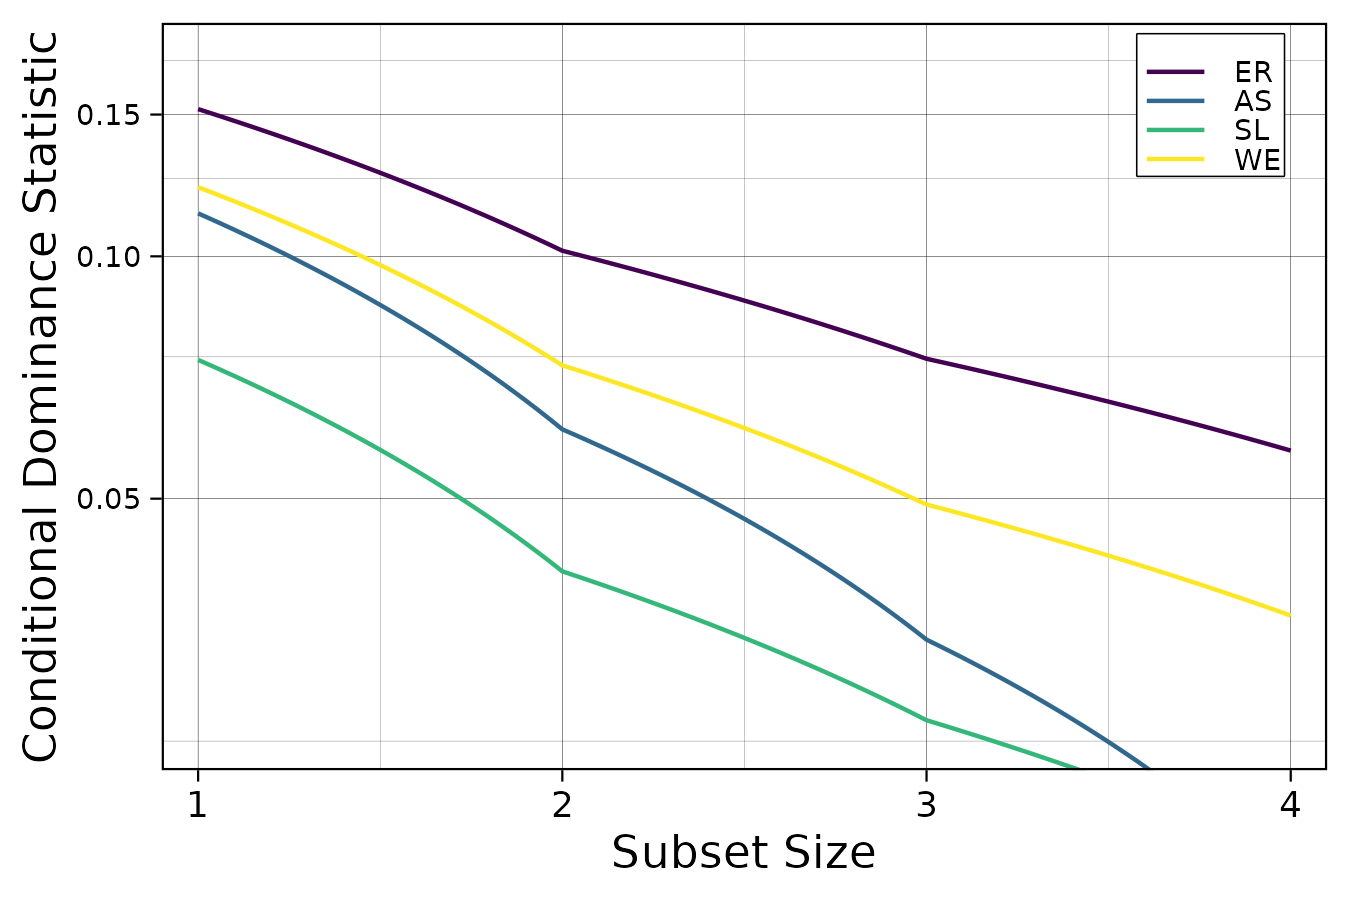
\includegraphics{includes/condit_gph}
	
	Figure X1 shows that $IV_4$ conditionally dominates all three of the other IVs.
	By contrast, the three other IVs have no conditional dominance relationships.
	This is because the three lines describing $IV_1$, $IV_2$, and $IV_3$'s conditional dominance statistics cross over one another between the three IV and all 4 IV in the model.
	
	It is worth noting that the ordering of the conditional dominance statistics at 4 IVs in the model for the LRM and CRM mirror the order of the standardized coefficient magnitudes ... whereas for 3 IVs or less in the model the ordering match the order of the correlations with the DV...
	
	The conditional dominance statistics reinforce the similarity across LRM and CRM DA results as the trends for each IV across numbers of IVs in the model are nearly identical.
	Again, the difference between LRM-based DA and CRM-based DA is primarily in the choice of fit metric and underlying predictive model; implementation between both is identical and, when the results are designed to be similar, the DA statistics produced are similar.
	
	The $R^2$ values in Table X5 can also be used to determine complete dominance of IVs over one another.  
	Because $IV_1$, $IV_2$, and $IV_3$ have no conditional dominance designations over one another, they cannot have complete dominance designations.
	$IV_4$ does conditionally dominate each of $IV_1$, $IV_2$, and $IV_3$; thus, $IV_4$ could possible also completely dominate each other IV.  
	The pattern of $R^2$ values in Table X5 shows that for both the LRM and CRM results, $IV_4$ completely dominates $IV_1$, $IV_2$, and $IV_3$.
	
	\subsubsection{Section Summary}
	
	This section intended to provide a detailed example of the estimation of both a LRM and CRM as well as DAs based on those models.
	The examples provided were based on generated data that were produced with the intention of being (reasonably) realistic as well as being as comparable as possible across LRM and CRM results.
	The data analytic examples of DA presented provide empirical evidence for the theoretical expectation that a LRM and CRM that are based on the same underlying causal structure should produce similar DA results.
	This demonstration thus serves to illustrate the straightforward generalization of DA from LRM to CRMs.
	
	Although DA with both LRM and CRMs can produce similar results when sharing an underlying causal structure, there are additional complexities to CRM estimation that do not have similar analogs with LRM given the data generating mechanisms underlying count DVs.
	The discussion of DA with CRMs turns, in next section, to a more extensive discussion of this additional complexity and when it can impact DA statistics and determinations.
	
	
	%this part below (other than final transition) needed in this section?
	The data for the analytic examples were generated using R \cite{R} using a combination of base R's \texttt{stats} package as well as the \texttt{MASS} package \cite{MASS}.  
	Other details of data generation for the reproducibility of the analysis can be found in Appendix X.  
	The section below transitions from discussing data generation processes to data analysis.
%	
%	\subsection{Base Relative Importance Results}
%	
%	The data generated above by data structure and DV distribution were submitted to separate DAs to produce a total of twelve different DAs.
%	The four DAs with each Normally distributed DV was based on linear regression.
%	The four DAs with each Poisson distributed DV was based on Poisson regression/generalized linear model with a log link and Poisson family.
%	The four DAs with each negative Binomial distributed DV was based on negative Binomial regression/generalized linear model with a log link and negative Binomial family.
%	The model parameter estimates for each of the twelve models DAs were also estimated but are not reported in this section as they are not a focus; these results are reported in Appendix X. 
%	The general dominance statistic results from each DA are presented in table X.
%	
%	
%		\subsubsection{Linear Model}
%	
%	The results from the linear model-based DA is, as noted above, most useful in this table as a comparison point for the other results computed from the CRMs.
%	The linear model is used as a comparison point as it is a better known model than most CRMs and is easier to work with mathematically.
%	The EU data structure is also intended to be a comparison point data structure representing idealized, if unrealistic, data conditions for estimation.
%	As such, I begin the interpretation of the results with the EU data.	
%	The idealized data structure represented by the EU condition produced results that were consistent with those which would be theoretically expected with identically distributed, uncorrelated IVs.  
%	Specifically, when there are no intercorrelations and the variance of the variable is 1, the expected $R^2$ value is the square of the coefficient (cite?).
%	The linear model results in Table X for the EU data structure follow this pattern well and show that general dominance statistic results, when there are no intercorrelations and equal variances, recover the theoretically expected $R^2$ values.  
%	Indeed, as is well known (cite?), DA is not a necessary procedure when IVs are not intercorrelated as the incremental $R^2$ values for each IV are tantamount to the general dominance statistics.
%	
%	% report the conditional dominance and complete stats too?
%	
%	The UU results vary from those obtained by the EU in that $V_4$, despite having a known coefficient value that is half that of $V_1$ obtained nearly the same general dominance statistic value.
%	As with the EU structure, UU's results are theoretically known.
%	For variables with unequal variances with no intercorrelations, the expected $R^2$ value is the square of the coefficient times the IV variance (cite?).
%	Hence, the expected general dominance statistics for $V_1$ and $V_4$ in the UU data structure were theoretically the same (i.e., $C_{V_1} = .2^2*1 = .1^2*4 = C_{V_4}$) however as realized in data as simulated in this manuscript, $V_1$ gained a slight edge and generally dominates $V_4$.
%	The results from the UU condition are intended to reinforce the idea that there are two 'routes' to importance with DA, the magnitude of the relationship between the IV and the DV as well as the variance of the IV.
%	Both relationship and variance contribute to the magnitude of the fit metric.
%	
%	% emphasize the variance and intercorrelations piece more above?  Maybe sufficient - just revisit
%	
%	The EC results for the linear model also vary from those obtained from the EU model by both increasing the total $R^2$ values obtained for each IV, in particular $V_3$ and $V_4$, but also by decreasing the relative differences between the IVs.
%	The increases in the values obtained by $V_3$ and $V_4$, despite their variance and known effect on $Y_{cont}$ being identical to EU, occur as a result of the intercorrelations between each IV.  
%	The introduction of the non-zero intercorrelations makes between IVs results in ambiguity about how the $R^2$ should be decomposed as the large effect $V_1$ is known to have on $Y_{cont}$ is now associated with the effects of the other three IVs when considering predicted values.  
%	That is, a change in $V_1$ is usually also associated with a change in $V_2$ (as they are correlated at .5 or share 25\% of their variance) and, to a lesser extent, also $V_3$ and $V_4$.
%	As a result of this correlation, predicted values on $Y_{cont}$ tend to move up or down together.
%	This shared change in predicted values makes it more difficult to tease apart to which variable should the change in predicted values, and thus improvement to explained variability when prediction improves, be attributed.
%	Previously less important IVs are then ascribed higher shares of the $R^2$ as the DA algorithm tends to resolve the ascription ambiguity by ascribing $R^2$ value to IVs based on weighted a weighted average of their $\Delta R^2$ across numbers of IVs in a sub-model (see equation ...).  
%	Ultimately, \emph{some} of the effect of an IV with a stronger effect on $Y_{cont}$ will be ascribed to those with less strong effects as is observed in Table X's EC results by contrast with EU given the ambiguity in ascription.
%	In addition, the total/model $R^2$ has increased given the intercorrelations ... reasons - artifact of way I made these? ...
%	Although the intercorrelations have increased the share of the $R^2$ ascribed to $V_3$ and $V_4$, it is important to note that, in this case, the rank order of the IVs does not change relative to the rank order in EU.
%	The results from the EC condition then emphasize that the intercorrelations between IVs increase the difficulty in ascribing $R^2$ to IVs which tends to benefit IVs with weaker relationships with the DV and penalize IVs with stronger relationships with the DV.	
%	
%	Finally, the UC results combine both the difficulty in ascribing $R^2$ to IVs of the EC condition with the unequal variances of the UU condition to produce a result that both substantially increased the total $R^2$ values attributed to each IV but also changed the rank order of the IVs such that $V_4$ generally dominates each other IV.
%	Overall, the results from the UC condition are similar to those obtained from the UU condition in that $V_1$ and $V_4$ are most important overall but, like the results from EC, the relative differences between the IVs' general dominance statistics have shrunk.
%	The UC condition is arguably the most realistic condition of the four data structures as variance differences and non-zero IV intercorrelations are common in collected data.
%	The UC condition is thus intended as a condition to show reflect the effect of realistic, but non-ideal, data conditions on DA results.
%	
%	The sections below transition to evaluating these same four data structures among DA results for the Poisson CRM with the recommended deviance $R^2$.  
%	A focus of the discussion will be on similarities and differences across models that are based on the same underlying data structures and DV predictive model.
%	
%	\subsubsection{Poisson Model}
%	
%	Before discussing the results from the Poisson model/$Y_{pois}$ DV, it is important to recall that $Y_{pois}$ is based on the save data structure as all the results based on $Y_{cont}$ and, in addition, is a direct translation of $Y_{cont}$ into a Poisson distributed variable. 
%	Thus, the results are intended to be as identical as possible across models to assist in comparability.
%	It is then not surprising to note that the Poisson model DA results show a similar pattern to those of the linear model of which they are an extension.
%	
%	...
%	
%	can be compared to the linear model results and reveal the same pattern
%	
%	Table X shows the effect of the intended differences across data structures as realized in the DA results.
%	
%	Table X shows stark differences between the data structures in terms of the dominance statistics obtained by each of the IVs.  The EU data structure
%	
%	The effect of the data structure is apparent in these results.  
%	The uncorrelated, equal variance results generally recovered the correct amount of explained variance for each IV.  
%	When introducing correlations to the model, ....
%	
%	Whereas there were clear differences between the data structures in terms of importance determination, the results across fit metrics within a model were quite similar.
%	Table X shows that the proportional contribution to the fit metric each IV was ascribed remained stable across fit metrics within a model.
%	For instance, $IV_1$s proportional contribution for the Poisson model...
%	Moreover, the dominance determinations did not differ across metrics within a model.
%	$IV_1$ completely dominated all other...
%	
%	\subsubsection{Negative Binomial Model}
%	
%	\subsubsection{Section Summary}
%	
%	The base relative importance section reported on the results of the linear, Poisson, and negative Binomial
%	
%	%	One way to interpret the results presented above is to suggest that relative importance determination for CRMs is insensitive to fit metric choice. 
%	%	Despite their similarities however, the explained variance $R^2$ values are consistently discrepant from the deviance $R^2$ values with the Poisson model producing values that were too high and the negative Binomial producing values that were too low. 
%	%	This result then suggests that the primary risk of using the explained variance $R^2$ as opposed to the deviance $R^2$ is in mis-characterizing the extent of predictive usefulness of the model as a whole, which affects the the numeric magnitudes or results obtained by the DA, but metric choice does not, itself, affect relative importance determinations.
%	
%	In the section below the focus moves to determining relative importance among CRMs with specific attention to cases where the DVs have unequal exposures to the count generating process.
	
	
\section{Additional Consideration for CRMs: Exposure}
	
	CRMs, as models of counts of discrete events, implicitly assume that the events realized in the data are derived from a data generating mechanism that had the same number of chances to observe events, or same number of trials, across observations.
	In CRMs, an observation with a count of 10 events is assumed to have had the same chance to get that count of 10 events as any other observation with 10 events.  
	The problem that arises when the number of chances to observe events is different across observations is more straightforward to discuss in the context of an example.
	Imagine that one of the observations with 10 events discussed above had 100 chances to observe an event but the other had 1,000 chances.
	These two counts of 10 then imply starkly different probabilities of observing an event (i.e., $\frac{10}{100} = .1$ and $\frac{10}{1000} = .01$).
	In data, such equifinality in counts from different underlying probabilities can arise from observations that are units reflecting populations of different sizes or units reflecting different time periods in which events could occur (i.e., unequal employment tenures).
	
	...
	
	CDMs can control for such unequal \emph{exposure} to the count generating conceptual phenomenon using what is known as an \emph{offset} term.  
	The offset term is usually assumed to be natural log transformed for a CDM and enters into the CDM with a coefficient of 1.
	The coefficient of 1 results in the count DV being transformed into a rate out of the offset variable.
	How the count DV is transformed into a rate with a coefficient of 1 follows from the following algebraic manipulations.
	First, consider a simple case where an intercept only model is fit with an offset such as $y = e^{offset + \beta}$.
	Recall that the offset term is the natural log of a variable, say, $o$.  
	Applying the natural log, the prior equation can be written as $\ln y = \ln o + \beta$.
	Re-arranging the $\ln o$ term results in $\ln y - \ln o = \beta$ which, given the properties of logarithms, is tantamount to $\ln \frac{y}{o} = \beta$.
	Therefore, the inclusion of a natural log transformed offset variable results in the count DV transforming into a rate.
	This offset transformation corrects for the issue discussed above as the 10 counts result in the correct underlying rate of .1 versus .01 for each observation.
	
	In large part, an offset adjustment serves to re-scale specific observations' predictions and has the biggest effect on CDM's intercept value; adjusting it back to reflect the correct average rate across observations.
	The offset can, however, affect the magnitude of estimated coefficients if the offset is correlated with an IV.  
	When the offset is correlated with an IV, then the IV may be both related to exposure to the count generating phenomenon as well as the rate of count generation broadly.
	Not including the offset can then bias the CDM and can have a notable impact on IV relative importance.
	How offsets affect CRM modeling and importance determination will also be explored further in the empirical examples below.
	
	A second consideration relevant to CDV models is the use of model offsets.  An offset is a variable that is intended to reflect \emph{exposure} or differences between observations in the capability for that observation to produce a count.  Offset variables are usually factors such as population sizes (cite) or exposure time windows (cite) that will affect the observations' counts and are known about different observations beforehand.  Offsets are included into the model with a coefficient of 1 and serve to make the CDV a rate as they adjust the count such that $e^{y_{i} - offset_{i}} = $
	
	
	
	In the sections below, each of the three complications regarding CDVs is discussed in greater detail with a focus on how each can affect the determination of relative importance.
	
\section{Multiple Equations}
	
	... Poisson vs alternatives ...
		
	Finally, a common model applied to CDVs are \emph{zero inflated} models that are recommended for use in modeling CDVs in many situations (see Figure 3 of \cite{blevins2015count}).  Zero inflated models offer a great deal of flexibility in evaluating the processes
	
	The flexibility of zero inflated models comes at the cost of greater complexity when considering how to evaluate the contributions IVs have to prediction as there are two predictive equations, the count-producing model and the zero-producing model, which need not have the same set of predictors.  As such, it may be necessary to examine parameter estimate relative importance (PERI; \cite{luchman2020relative}) as opposed to independent variable relative importance (IVRI) when examining 

	\subsection{Modeling with Exposure}
	
	...
	
	\subsection{Modeling with Zero-inflation}
	
	...
	
	% poisson
	
	Poisson and linear regression share many similarities and, as a result of these similarities, often give similar answers when a count DV is applied to either model.
	Indeed the DA results for the Poisson model with the deviance $R^2$ are strikingly similar to those obtained from the Gaussian DV DA both in terms of the magnitudes of the deviance R2.  
	This result is as expected in that the Poisson results are an extension of the Gaussian DV-based results and the deviance $R^2$ is a direct generalization of the explained variance $R^2$ to generalized linear models.
	
	When applying
	
	...
	
	
	CDV models are complex, inherently multiplicative (note that it is possible to estimate them as non-multiplicative - but this is rarely done) models that require the use of estimation techniques such as maximum likelihood to obtain parameter estimates and sampling variances.
	It is helpful to discuss some of the nuances of how these models are estimated to understanding the implications of these complexities for DA.
	Hence, in the sections to come, I discuss aspects 
%
%	\subsection{Poisson Regression: The Most Basic Case}
%	
%	The most conceptually simple CDV model is the Poisson regression.  
%	The Poisson regression's log likelihood is a sum of three components as is shown below in (can I reference this equation?).
%	
%	\begin{equation}
%		\ln L = \sum_{i=1}^{N} xb_{i}y_{j} - (\ln (y_{i}!) + e^{xb_{i}})
%	\end{equation}
%
%	Where $xb_{i}$ refers to a respondent's untransformed/linear predicted value from the Poisson regression.  
%	Of note with this log-likelihood is the division into two separate components.  
%	On the one hand, the log-likelihood increases, with the $xb_{i}y_{j}$ term.  
%	Hence, the product of the observed CDV value and the predicted value for a respondent contributes directly to the log-likelihood and indicates better fit to the data.
%	On the other hand, the second set of terms, $\ln (y_{i}!) + e^{xb_{i}}$ decrease the log-likelihood.  
%	Thus, has the log factorial of the CDV increases and as the exponential function of the predicted values increase without a concomitant increase in the $xb_{i}y_{j}$.
%	
%	For example consider a respondent with a CDV value of 5.  
%	The best fit to this value would be a transformed predicted value of 5 or an untransformed/linear predicted value of $e^{5} = -1.740$.  
%	When applied to the log-likelihood function, the value obtained is $5*-1.740 - \ln (5) + e^{-1.740} = -1.740$ or untransformed/linear predicted value.
%	By contrast, two hypothetical less ideal predicted values might be 4 and 6.  
%	In both cases, the log-likelihood values diverge from the best fitting one and increase, indicating a lower likelihood.
%	Specifically, 4 gives $5*\ln (4) - \ln (5) + 4 = -1.856$ and 6 gives $5*\ln (6) - \ln (4) + 6 = 1.829$...
%	This also shows an important point about the Poisson log likelihood--that it is not symmetric around the best fitting value.  
%	By contrast, ordinary least squares regression would penalize both 4 and 6 as squared deviations of 1 from the line of best fit (footnote that logged DV can do this too - but the loglik is still symmetrical and the model is now fitting the mean of a transformed DV as opposed to the original DV).
%	That the model fit to the data is asymmetrical has implications for assessing fit to the model that will be discussed in greater detail later.
%	
%	\subsection{Negative Binomial: A More Complex and Flexible Case}
%	
%	A constraint with the Poisson model is that it has only a single parameter estimated from the data, it's mean.  The variance of the Poisson distribution is, by assumption, identical to the mean.
%	
%	One way to extend on the Poisson to make it more flexible is to conceptualize the mean of the Poisson distribution as a random variable.  If the mean of the Poisson is conceptualized as Gamma distributed, the hybrid Poisson-Gamma distribution can be reduced to a unique distribution called the negative Binomial.
%	
%	The negative Binomial model is a more complex generalization of the Poisson that relaxes the assumption that the variance and mean are identical
%	
%	...negative binomial...
%	
%	\begin{equation}
%		\ln L = \sum_{i=1}^{N} \ln (\Gamma (\frac{1}{\alpha} + y_{i}) ) + m- (\ln (y_{i}!) + e^{xb_{i}})
%	\end{equation}
%
%	
%
%	% rework below
%
%	In applying DA to CDVs, many readers might question whether there is a need to use methods other than the standard linear regression with the explained variance $R^2$ metric.
%	
%	Although CDV models share a number of similarities with continuous DVs, CDVs and the models designed to work with them are a distinct subset of generalized linear models and behave differently than linear regression in ways that  \emph{(cite Blevins and summarize somewhere around here)}.
%	
%	One similarity across count and continuous DVs is that, as the mean of a CDV variable increases, it grows increasingly good at being approximated with a Normal distribution \emph{(cite!)}.  
%	This points to an important difference when applied to CDVs with rare events in that the distributions for count and continuous DVs diverge notably when the mean is nearer 0 (example here?).  
%	Such divergence results in important differences to model-to-data fit that not only affects the model fit metric's value overall but also how specific IVs explain variation in the CDV.  
%	In particular, CDVs are discrete, non-negative integers and, accordingly, CDV models are discrete probability distributions that accommodate non-negative integers.  
%	Normal distributions are continuous
%	
%	
%	
%
%	Applying DA to CDVs
%
%	% note to self - lean on Blevins, Tsang, and Spain (2014) for this discussion...
%
%	A useful first step toward defining recommended practice for applying DA to CDVs is to understand how CDV models differ from linear models.
%	Differences between CDV and linear models affect model estimation and how relative importance among IVs should be determined.	
%	One substantial difference between CDV models such as the Poisson from linear models is in the functional form of the model. 
%	In a linear model, the magnitude of the regression coefficient for an IV reflects the expected change in the DV given one unit of change in the IV. 
%	By contrast, CDV models most often use a log-linear linking function.
%  	In a log-linear link model like the Poisson, the coefficients are estimated using from the data as though they were transformed using a natural logarithm.  This implied transformation, or linking function, results in the CDV effectively ranging over all real numbers just like a continuous DV is expected to in linear regression.
%  	
%  	  	% equation here?%
%  	\begin{equation}
%  		ll = \frac{1}{1}
%  	\end{equation}
%  	
%  	Although the CDV is implied to range over all real numbers in the estimation algorithm, the observed CDV is not changed and the predicted values from the CDV model are in log-linear units as opposed to those of the CDV (i.e., counts of the event).  	
%  	In order to produce meaningful predicted values, CDV models need to back-translate their predicted values to the metric of the CDV.  The back-translation applies an anti-log or exponential function to the predicted values.
%  	 
%  	the natural logarithm linking function used to translate the predicted values
%  	model from a linear model back to the original count metric results in a one unit change in the IV producing a different magnitude of change to the dependent variable depending on where on the continuum of the dependent variable the change is located. 
%
%	The log-linear nature of the coefficients produced by CDV models make the difficult to interpret directly. 
%	Typically, CDV coefficients are translated using an exponential function to produce \emph{Incidence Rate Ratios} or \emph{IRRs}.  
%	that naturally produce multiplicative effects across the range of each IV.
%
%	The naturally multiplicative functional form of CDV models makes the explained-variance $R^2$ metric less useful for DA.  This is because CDVs are not guaranteed to produce an increase to the explained-variance $R^2$ as more IVs are added to the model \cite{}.  
%	
%	There are pseudo-$R^2$s that are better able to characterize model fit for CDVs.  
%	
%	
%	\begin{equation}
%		\ln{y} = \sum{\beta_{x_i}}
%	\end{equation}
%
%	\subsection{Parameter Estimation Results}
%
%The data analysis begins where all relative importance analysis should, with parameter estimation using the statistical model appropriate for each DV.  
%Relative importance analysis is an extension of parameter estimation (cite!) that provides additional, useful information about the model and data.  
%As such, relative importance analysis results should be interpreted in light of the parameter estimates produced by the model that is being dominance analyzed.  
%The goal of this section is to highlight similarities and differences between the models' results across the four data structures with attention to each data structure's effect parameter estimate magnitudes. 
%
%\subsubsection{Base Model Results}
%
%This subsection discusses the parameter estimates obtained from the Normal, Poisson, and negative Binomial distributed DVs across all four data structures.  
%Note that descriptive statistics for the IVs and DVs are reported in Appendix X.  The results from the four models estimated on the Normal DVs are listed below in Table X.
%
%%
\begin{tabular}[t]{llrrrrrrrrrrrrrrrrrrrrrrrrrrrrrrrr}
\toprule
Parameter & Component & Coefficient.Model 1 & SE.Model 1 & CI.Model 1 & CI\_low.Model 1 & CI\_high.Model 1 & t.Model 1 & df\_error.Model 1 & p.Model 1 & Coefficient.Model 2 & SE.Model 2 & CI.Model 2 & CI\_low.Model 2 & CI\_high.Model 2 & t.Model 2 & df\_error.Model 2 & p.Model 2 & Coefficient.Model 3 & SE.Model 3 & CI.Model 3 & CI\_low.Model 3 & CI\_high.Model 3 & t.Model 3 & df\_error.Model 3 & p.Model 3 & Coefficient.Model 4 & SE.Model 4 & CI.Model 4 & CI\_low.Model 4 & CI\_high.Model 4 & t.Model 4 & df\_error.Model 4 & p.Model 4\\
\midrule
(Intercept) & conditional & 0.0026888 & 0.0030786 & 0.95 & -0.0033452 & 0.0087228 & 0.8733959 & 99995 & 0.3824494 & 0.0034259 & 0.0030518 & 0.95 & -0.0025555 & 0.0094073 & 1.122598 & 99995 & 0.2616109 & 0.0000505 & 0.0030863 & 0.95 & -0.0059987 & 0.0060997 & 0.016372 & 99995 & 0.9869376 & 0.0038046 & 0.0030342 & 0.95 & -0.0021424 & 0.0097515 & 1.253909 & 99995 & 0.2098780\\
V1 & conditional & 0.2002413 & 0.0030855 & 0.95 & 0.1941937 & 0.2062888 & 64.8973270 & 99995 & 0.0000000 & 0.1970549 & 0.0036431 & 0.95 & 0.1899144 & 0.2041953 & 54.089693 & 99995 & 0.0000000 & 0.2022451 & 0.0030979 & 0.95 & 0.1961733 & 0.2083168 & 65.285300 & 99995 & 0.0000000 & 0.2031623 & 0.0036134 & 0.95 & 0.1960802 & 0.2102445 & 56.224975 & 99995 & 0.0000000\\
V2 & conditional & 0.0989537 & 0.0030765 & 0.95 & 0.0929238 & 0.1049836 & 32.1643365 & 99995 & 0.0000000 & 0.1039673 & 0.0036471 & 0.95 & 0.0968189 & 0.1111156 & 28.506473 & 99995 & 0.0000000 & 0.1009850 & 0.0027595 & 0.95 & 0.0955764 & 0.1063935 & 36.595587 & 99995 & 0.0000000 & 0.1000512 & 0.0032422 & 0.95 & 0.0936965 & 0.1064058 & 30.859141 & 99995 & 0.0000000\\
V3 & conditional & 0.0153902 & 0.0030612 & 0.95 & 0.0093903 & 0.0213901 & 5.0274986 & 99995 & 0.0000005 & 0.0224097 & 0.0036388 & 0.95 & 0.0152777 & 0.0295417 & 6.158540 & 99995 & 0.0000000 & 0.0200877 & 0.0025219 & 0.95 & 0.0151447 & 0.0250306 & 7.965211 & 99995 & 0.0000000 & 0.0155381 & 0.0029455 & 0.95 & 0.0097650 & 0.0213111 & 5.275232 & 99995 & 0.0000001\\
V4 & conditional & -0.0205982 & 0.0030689 & 0.95 & -0.0266132 & -0.0145831 & -6.7118048 & 99995 & 0.0000000 & -0.0202537 & 0.0036526 & 0.95 & -0.0274127 & -0.0130947 & -5.545043 & 99995 & 0.0000000 & -0.0213533 & 0.0021843 & 0.95 & -0.0256345 & -0.0170720 & -9.775681 & 99995 & 0.0000000 & -0.0138422 & 0.0025663 & 0.95 & -0.0188720 & -0.0088124 & -5.393934 & 99995 & 0.0000001\\
\bottomrule
\end{tabular}

%
%The effects of data structure on estimation for Normally distributed variables with linear regression are well-known and the results in Table X are, as a result, consistent with extant research in showing that these data tended to recover the correct parameter estimates.
%
%...
%
%data generated were a rather large population size (100,000) and our model was correctly specified.  
%
%Hence, it is not a surprise that the known model parameters were recovered very well from the data across all four data structures and models.
%
%Recall that the true parameters were .2 for $X_1$, .15 for $X_2$, .125 for $X_3$, and .1 for $X_4$.  
%Also recall that these linear regression equations underlie the generation of both the Poisson and negative Binomial DVs.  
%I expect then that the linear regression results will serve as a useful comparison point for the CRM parameter estimation results.
%
%%
\begin{tabular}[t]{llrrrrrrrrrrrrrrrrrrrrrrrrrrrrrrrr}
\toprule
Parameter & Component & Log-Mean.Model 1 & SE.Model 1 & CI.Model 1 & CI\_low.Model 1 & CI\_high.Model 1 & z.Model 1 & df\_error.Model 1 & p.Model 1 & Log-Mean.Model 2 & SE.Model 2 & CI.Model 2 & CI\_low.Model 2 & CI\_high.Model 2 & z.Model 2 & df\_error.Model 2 & p.Model 2 & Log-Mean.Model 3 & SE.Model 3 & CI.Model 3 & CI\_low.Model 3 & CI\_high.Model 3 & z.Model 3 & df\_error.Model 3 & p.Model 3 & Log-Mean.Model 4 & SE.Model 4 & CI.Model 4 & CI\_low.Model 4 & CI\_high.Model 4 & z.Model 4 & df\_error.Model 4 & p.Model 4\\
\midrule
(Intercept) & conditional & -0.03429 & 0.00327 & 0.95 & -0.04070 & -0.02789 & -10.48655 & Inf & 0 & -0.06388 & 0.00336 & 0.95 & -0.07046 & -0.05729 & -19.00151 & Inf & 0 & -0.05711 & 0.00334 & 0.95 & -0.06366 & -0.05056 & -17.08449 & Inf & 0 & -0.11018 & 0.00350 & 0.95 & -0.11704 & -0.10332 & -31.47987 & Inf & 0\\
V1 & conditional & 0.18262 & 0.00318 & 0.95 & 0.17640 & 0.18884 & 57.51537 & Inf & 0 & 0.18175 & 0.00377 & 0.95 & 0.17436 & 0.18914 & 48.20979 & Inf & 0 & 0.18142 & 0.00317 & 0.95 & 0.17522 & 0.18763 & 57.29487 & Inf & 0 & 0.18531 & 0.00375 & 0.95 & 0.17796 & 0.19267 & 49.40490 & Inf & 0\\
V2 & conditional & 0.13493 & 0.00316 & 0.95 & 0.12875 & 0.14112 & 42.75617 & Inf & 0 & 0.13887 & 0.00377 & 0.95 & 0.13148 & 0.14626 & 36.83888 & Inf & 0 & 0.13819 & 0.00258 & 0.95 & 0.13314 & 0.14325 & 53.61428 & Inf & 0 & 0.13656 & 0.00308 & 0.95 & 0.13053 & 0.14259 & 44.39591 & Inf & 0\\
V3 & conditional & 0.10691 & 0.00314 & 0.95 & 0.10075 & 0.11307 & 34.02206 & Inf & 0 & 0.11344 & 0.00377 & 0.95 & 0.10606 & 0.12083 & 30.10639 & Inf & 0 & 0.11374 & 0.00224 & 0.95 & 0.10936 & 0.11812 & 50.87253 & Inf & 0 & 0.10977 & 0.00265 & 0.95 & 0.10457 & 0.11496 & 41.42294 & Inf & 0\\
V4 & conditional & 0.09054 & 0.00315 & 0.95 & 0.08437 & 0.09671 & 28.76795 & Inf & 0 & 0.08951 & 0.00378 & 0.95 & 0.08211 & 0.09692 & 23.69032 & Inf & 0 & 0.08998 & 0.00158 & 0.95 & 0.08688 & 0.09308 & 56.94384 & Inf & 0 & 0.09378 & 0.00189 & 0.95 & 0.09008 & 0.09749 & 49.64825 & Inf & 0\\
\bottomrule
\end{tabular}

%
%Numerically, the Poisson results look rather similar to the linear regression results as was intended.  
%Indeed, the linear regression prediction equation (with error) was used to generate the underlying Poisson distributed variable and both had the same underlying variance of 1.
%A further similarity between the linear and Poisson results is that the coefficients obtained across data structures were nearly identical with the exception of the intercept.
%
%%
\begin{tabular}[t]{llrrrrrrrrrrrrrrrrrrrrrrrrrrrrrrrr}
\toprule
Parameter & Component & Log-Mean.Model 1 & SE.Model 1 & CI.Model 1 & CI\_low.Model 1 & CI\_high.Model 1 & z.Model 1 & df\_error.Model 1 & p.Model 1 & Log-Mean.Model 2 & SE.Model 2 & CI.Model 2 & CI\_low.Model 2 & CI\_high.Model 2 & z.Model 2 & df\_error.Model 2 & p.Model 2 & Log-Mean.Model 3 & SE.Model 3 & CI.Model 3 & CI\_low.Model 3 & CI\_high.Model 3 & z.Model 3 & df\_error.Model 3 & p.Model 3 & Log-Mean.Model 4 & SE.Model 4 & CI.Model 4 & CI\_low.Model 4 & CI\_high.Model 4 & z.Model 4 & df\_error.Model 4 & p.Model 4\\
\midrule
(Intercept) & conditional & -0.08308 & 0.00535 & 0.95 & -0.09355 & -0.07260 & -15.54090 & Inf & 0 & -0.15130 & 0.00529 & 0.95 & -0.16168 & -0.14093 & -28.58388 & Inf & 0 & -0.13849 & 0.00533 & 0.95 & -0.14893 & -0.12804 & -25.98065 & Inf & 0 & -0.27272 & 0.00525 & 0.95 & -0.28301 & -0.26243 & -51.93894 & Inf & 0\\
V1 & conditional & 0.28582 & 0.00535 & 0.95 & 0.27534 & 0.29629 & 53.46381 & Inf & 0 & 0.28415 & 0.00617 & 0.95 & 0.27205 & 0.29625 & 46.03097 & Inf & 0 & 0.28456 & 0.00526 & 0.95 & 0.27426 & 0.29487 & 54.10380 & Inf & 0 & 0.30633 & 0.00585 & 0.95 & 0.29487 & 0.31780 & 52.35033 & Inf & 0\\
V2 & conditional & 0.20828 & 0.00530 & 0.95 & 0.19789 & 0.21866 & 39.30780 & Inf & 0 & 0.21842 & 0.00616 & 0.95 & 0.20635 & 0.23048 & 35.48152 & Inf & 0 & 0.21472 & 0.00427 & 0.95 & 0.20634 & 0.22309 & 50.25707 & Inf & 0 & 0.21600 & 0.00479 & 0.95 & 0.20662 & 0.22539 & 45.13136 & Inf & 0\\
V3 & conditional & 0.16658 & 0.00526 & 0.95 & 0.15626 & 0.17690 & 31.64090 & Inf & 0 & 0.17870 & 0.00614 & 0.95 & 0.16666 & 0.19074 & 29.08685 & Inf & 0 & 0.17871 & 0.00370 & 0.95 & 0.17145 & 0.18597 & 48.23773 & Inf & 0 & 0.17668 & 0.00412 & 0.95 & 0.16859 & 0.18476 & 42.84480 & Inf & 0\\
V4 & conditional & 0.13695 & 0.00527 & 0.95 & 0.12663 & 0.14728 & 25.99445 & Inf & 0 & 0.14662 & 0.00616 & 0.95 & 0.13455 & 0.15869 & 23.80613 & Inf & 0 & 0.14335 & 0.00262 & 0.95 & 0.13820 & 0.14849 & 54.63271 & Inf & 0 & 0.15291 & 0.00295 & 0.95 & 0.14714 & 0.15869 & 51.91722 & Inf & 0\\
\bottomrule
\end{tabular}

%
%The negative Binomial regression results, by contrast to the Poisson, were numerically less similar to the linear regression and more noticeably sensitive to data conditions during model estimation.
%For instance, the negative Binomial results tended to produce larger coefficients when the variables were both correlated and had unequal variances.
%The next section shifts to focus on the effect of the model, data structure, and fit metric chosen have on the determination of relative importance.
%
%\subsubsection{Offset Models}
%
%\subsubsection{Zero-inflated Models}


\bibliography{CountDominance.bib}
\bibliographystyle{mslapa}
	
\end{document}